\documentclass[journal,trans]{IEEEtran}
\usepackage[utf8]{inputenc}
\usepackage{graphicx}
\usepackage{apacite}



\title{Practice 3.Go-Back-N ARQ implementation using CRC}
\date{June 2021}
\author{*Granados Bello Martin Alejandro
*González García Alan Alberto
*Vega Barbosa Angel Josuhe 
*Hernán Bonilla Jesús Hernán
*Gutiérrez Herrera Andrea
\thanks{Student at the IPN-UPIITA university }}



\begin{document}

\maketitle

\begin{abstract}
The Data Link layer is responsible for transferring messages (frames) over the physical channel. At the same time, it transforms an error-prone physical channel into a virtually error-free logical link.

In wide-area networks, the Link layer provides a connection service via point-to-point links between each pair of (connected) network nodes. It performs the functions and procedures necessary to establish, maintain and carry out these connections.

CRC stands for cyclic redundancy check, also called polynomial code checksum. In Spanish, control de redundancia cíclica or cyclic redundancy check.
CRC is a function designed to detect accidental changes in computer data and is commonly used in digital networks and storage devices (such as hard disks).
CRC was created by W. Wesley Peterson in 1961; the 32-bit polynomial used in Ethernet (and other standards) CRC functions was published in 1975.
The CRC is very popular because it is simple to implement, easy to analyze mathematically and is very good at detecting errors caused by noise in the transmission channels.

\end{abstract}

\section{Introduction}

The motivation of the practice It is known that the OSI model has been the reference model in
recent years, for many telecommunications systems. Hence, it is important to
understand and identify each of the layers that a telecommunications system
has, not just in theory, but in real applications too.

The objective is Identify, design and develop a basic 2.4GHz RF telecomunication
system based on the physical and link layer using CRC and ARQ protocols.
\section{\textbf{Arduino Module}}
The arduino Uno is a board based on an Atmega328 microcontroller. It has 14 digital input / output pins (of which 4 can be used for PWM outputs), 6 analog inputs, a 16 MHz ceramic resonator, a female type USB connector, a Power supply Jack, an ICSP connector and a reset button.
It has everything you need to handle the controller, we simply connect to the computer through the USB cable or an external power source, which can be an AC-DC adapter or a battery, it should be noted that if it is powered through the USB cable in the computer does not need an external source.
\cite{casco2014raspberr}

To program the board you need the Arduino IDE.

\subsection{\textbf{arduino module specifications }}
\begin{itemize}
  \item \textbf{ Microcontroller: ATmega328}
    \item \textbf{ Operating Voltage: 5v }
    \item \textbf{ Input Voltage (Recommended): 7 - 12 v }
    \item \textbf{ Digital Input / Output Pins: 14 (Of which 6 are PWM outputs)}
	\item \textbf{ Analog Input Pins: 6} 
	\item \textbf{ Flash memory: 32 KB (ATmega328) of which 0.5 KB is used by Bootloader.} 
    \item \textbf{ SRAM: 2 KB (ATmega328)} 
    \item \textbf{ EEPROM: 1 KB (ATmega328)} 
    \item \textbf{ Clock Speed: 16MHZ} 

\end{itemize}
\begin{figure}[h]
    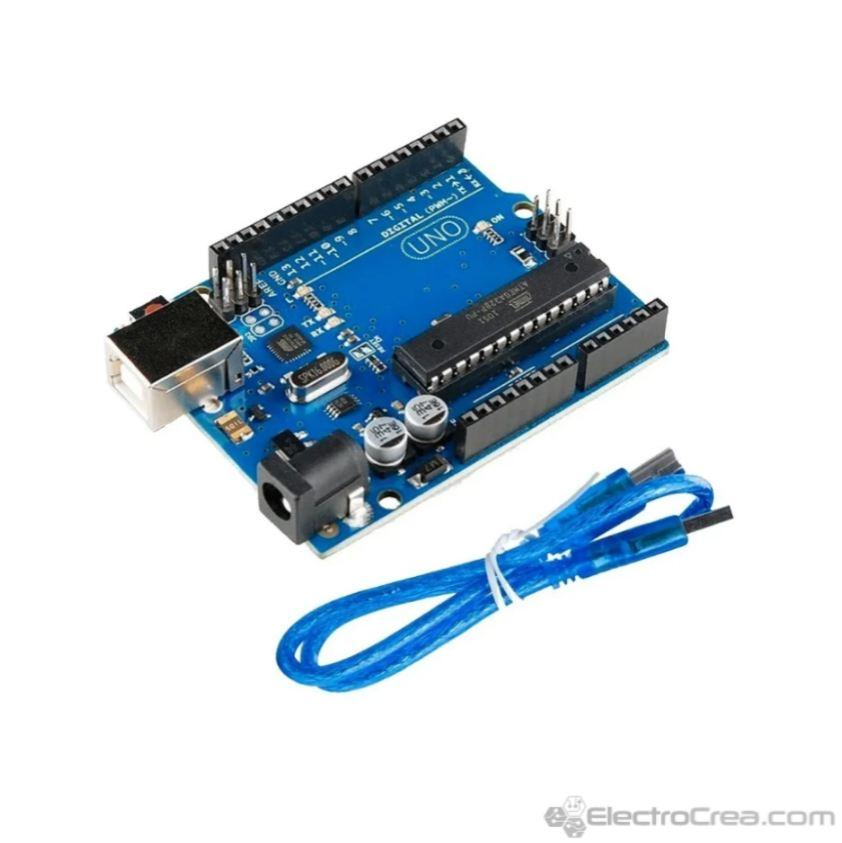
\includegraphics[width=0.3\textwidth]{ArduinoUno.jpg}
    \centering
    \caption{Arduino UNO}
    \label{fig:my_label}
\end{figure}

\section{\textbf{module NRF24L01}}
This module uses Nordic Semiconductor's new 2.4GHz transceiver, the NRF24L01 that operates in the 2.4GHz band (Industrial, Scientific and Medical) and has new features, such as its ultra low power consumption (ULP). The Nordic nRF24L01 + chip integrates a complete 2.4Ghz transceiver, RF synthesizer, and logic such as the improved ShockBurst ™, which is a hardware protocol accelerator for SPI communication with microcontroller.

The module has 8 pins (male headers) through which it is powered (3.3V) and communicates through SPI.

It has a power amplifier circuit (PA), a low noise amplifier circuit (LNA) as well as an SMA antenna that allows it to achieve a range of up to 1000m in field of view.

\subsection{\textbf{module NRF24L01 specifications }}
\begin{itemize}
  \item \textbf{Power supply: 1.9 ~ 3.6V}
    \item \textbf{ IO port working voltage: 0 ~ 3.3v / 5v (Tolerant to 5V)}
  \item \textbf{Current Consumption: 115 mA}
  \item \textbf{ Transmission rate: +20 dBm}
  \item \textbf{ Sensitivity reception: -95dBm at 1Mbps} 
  \item \textbf{ Transmission range: 1000m in open area} 
  \item \textbf{Operates in the 2.4 GHz ISM band, so it does not need a license and is free worldwide} 
    \item \textbf{3 Selectable Data } 
    \item \textbf{ Ultra low power consumption, able to last for years using a battery} 

\end{itemize}

\begin{figure}[h]
    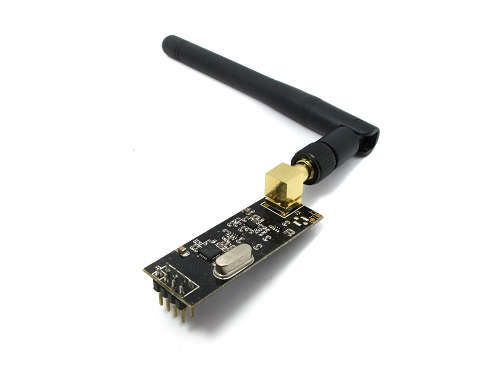
\includegraphics[width=0.3\textwidth]{Modulo.jpg}
    \centering
    \caption{Modulo NRF24L01}
    \label{fig:my_label1}
\end{figure}

\section{\textbf{ARQ protocol}}
The Data Link layer is responsible for the transfer of messages (frames) through the physical channel. At the same time, it transforms an error-prone physical channel into a virtually error-free logical link.\cite{zambrano2015estudio}

In long-range networks, the Link layer provides a connection service through point-to-point links between each pair of network nodes (that are connected). It performs the functions and procedures necessary to establish, maintain and carry out these connections.
\cite{caire2001throughput}
ARQs like Stop-and-Wait, Go-Back-N, and Selective Repeat are protocols that ensure reliable data transfer. For this, they use codes such as CRC to determine integrity (ED) and send ACKs or NAKs if the sent packets arrive, and if they do not arrive or arrive incorrectly, they request a retransmission.
A variation of these protocols are the ARQ-Hybrids, which in addition to checking the integrity of the received packets, provide information that allows correcting some errors (FEC), without the need to request extra data. This results in no need for a channel back to the transmitter or to avoid retransmissions, but at the cost of higher bandwidth. For this reason they are more widely used where broadcasting is very expensive or technically difficult. It can be summarized in that when the
Link quality is poor, it is more convenient to use ARQ-hybrids, but when link quality is good, throughput decreases. Cases where this is required are in wireless connections of mobile phones such as UMTS (3G-4G) and mobile WiMAX (WiFi).

\subsection{\textbf{ ARQ with stop and wait }}

The Stop-and-wait method is a type of ARQ protocol for controlling errors in communication between two hosts based on the sending of frames or packets, so that once a packet is sent, it is not it sends the next packet until the corresponding ACK (reception confirmation) is received and in case of receiving a NACK (reception rejection) the previous packet is forwarded.

\begin{figure}[h]
    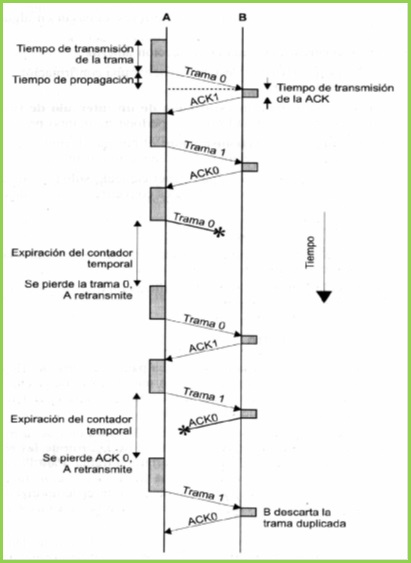
\includegraphics[width=0.3\textwidth]{ARQ-SaW.jpg}
    \centering
    \caption{ARQ Stop and Wait}
    \label{fig:my_label2}
\end{figure}

\subsection{\textbf{ ARQ with turn back N}}

It is almost the same as the previous method except that this technique has a sliding window. The frames received (either with RRnº of the next frame, or with piggy-backing).

If the receiver detects an error, it can now notify the sender by means of a negative confirmation message (REJect).

\begin{figure}[h]
    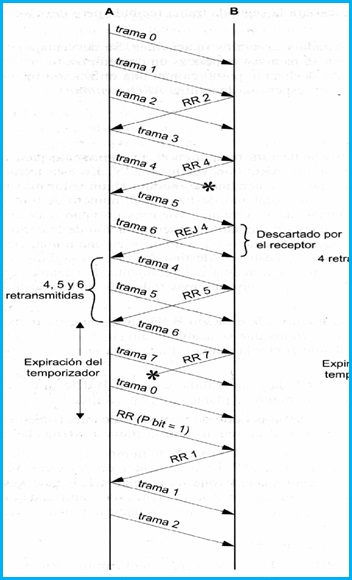
\includegraphics[width=0.3\textwidth]{ARQ-TurnB.jpg}
    \centering
    \caption{ARQ with turn back N}
    \label{fig:my_label3}
\end{figure}

\subsection{\textbf{ ARQ with selective rejection}}

It avoids the retransmission of correctly received frames when there has been an error in the preceding ones. Now when the receiver detects an error in the received frame, instead of sending REJ, it transmits the SREJ (Selective REJect) frame that orders its retransmission. The sender obeys, but continues the communication from where it left off, without assuming that the rest of the frames sent and still pending confirmation have also been erroneous.

\begin{figure}[h]
    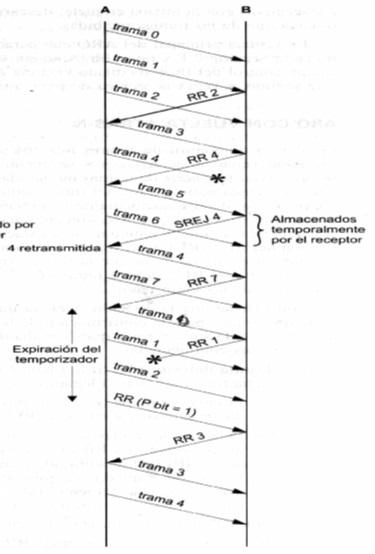
\includegraphics[width=0.3\textwidth]{ARQ-rechazo.jpg}
    \centering
    \caption{ARQ with selective rejection}
    \label{fig:my_label4}
\end{figure}

\section{\textbf{Cyclic redundancy check}}
A cyclic redundancy check (CRC) is an error-detecting code commonly used in digital networks and storage devices to detect accidental changes to raw data. Blocks of data entering these systems get a short check value attached, based on the remainder of a polynomial division of their contents. On retrieval, the calculation is repeated and, in the event the check values do not match, corrective action can be taken against data corruption. CRCs can be used for error correction (see bitfilters).

CRCs are so called because the check (data verification) value is a redundancy (it expands the message without adding information) and the algorithm is based on cyclic codes. CRCs are popular because they are simple to implement in binary hardware, easy to analyze mathematically, and particularly good at detecting common errors caused by noise in transmission channels. Because the check value has a fixed length, the function that generates it is occasionally used as a hash function.

To compute an n-bit binary CRC, line the bits representing the input in a row, and position the (n + 1)-bit pattern representing the CRC's divisor (called a "polynomial") underneath the left end of the row.

In this example, we shall encode 14 bits of message with a 3-bit CRC, with a polynomial x3 + x + 1. The polynomial is written in binary as the coefficients; a 3rd-degree polynomial has 4 coefficients (1x3 + 0x2 + 1x + 1). In this case, the coefficients are 1, 0, 1 and 1. The result of the calculation is 3 bits long, which is why it is called a 3-bit CRC. However, you need 4 bits to explicitly state the polynomial.


\section{\textbf{Tasks}}
Within a radius of approximately 13 meters, the following packet sending and receiving tests were performed, with the implementation of CRC and the ARQ GO BACK N protocol, thus obtaining results more faithful to what it would be in its functionality in the field or any real test.

\subsection{\textbf{Actual successful packets arrival and total packets sent.}}
\begin{figure}[h]
    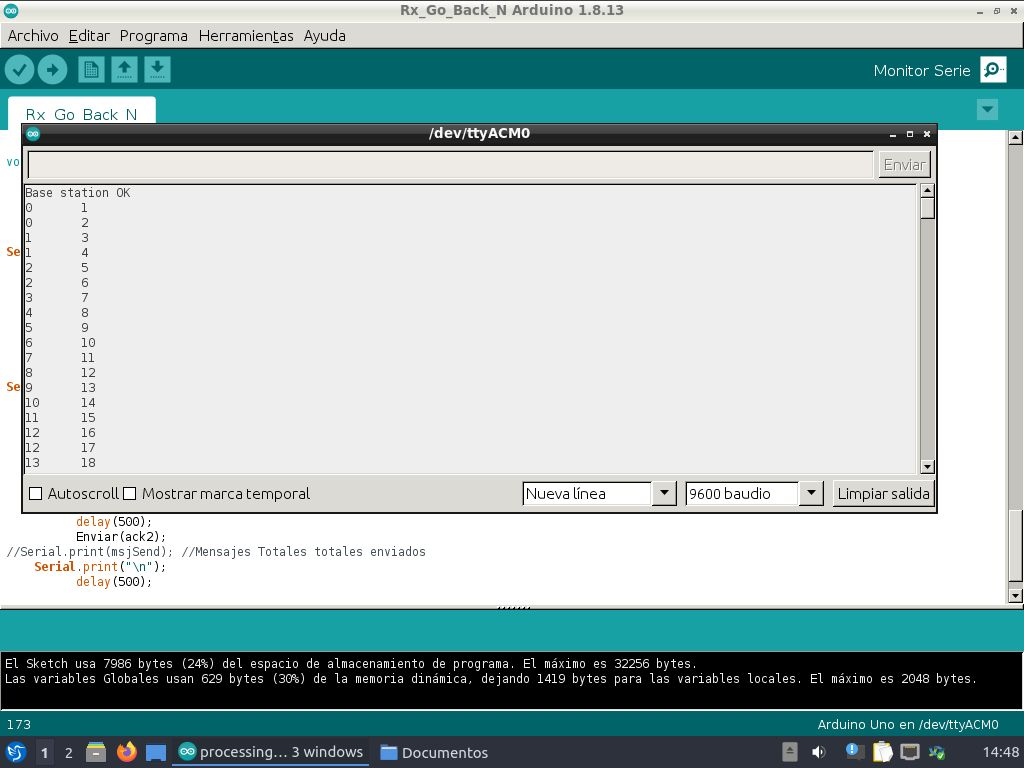
\includegraphics[width=0.3\textwidth]{ex1.jpeg}
    \centering
    \caption{Viewing the result of GO-BACK-N code}
    \label{fig:my_label5}
\end{figure}

\subsection{\textbf{Plot for successful packets arrival and total packets sent.}}
\begin{figure}[h]
    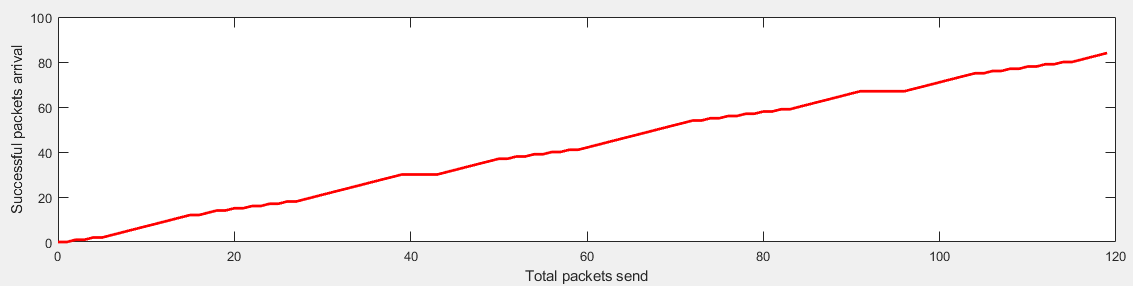
\includegraphics[width=0.3\textwidth]{plot1.PNG}
    \centering
    \caption{succesful packets delay (AoI) Vs actual succesful packets arrival time}
    \label{fig:my_label6}
\end{figure}

\begin{figure}[h]
    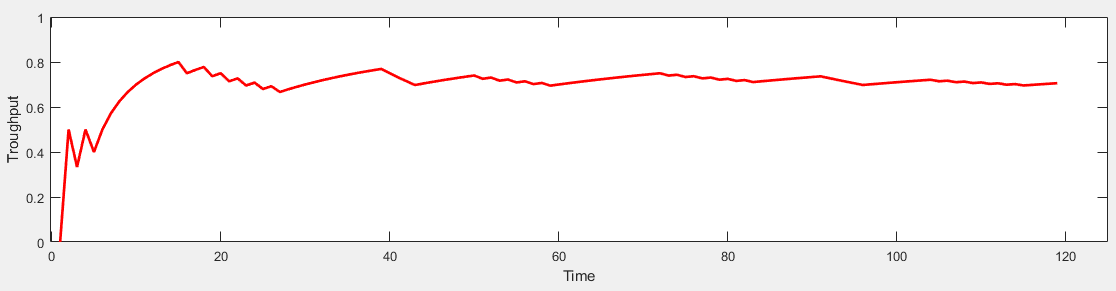
\includegraphics[width=0.3\textwidth]{plot2.PNG}
    \centering
    \caption{Troughput vs Time}
    \label{fig:my_label6}
\end{figure}
With the small-scale samples that we have taken at an interval of approximately 2 minutes, it is not possible to fully appreciate the differences between them, but we can highlight a higher percentage of packets received successfully, given that the protocol that has been implemented uses a window of size 2 and this allows sending a greater number of packets in the same amount of time.
\subsection{\textbf{Comparison of the plot of practice 2 with the plot of this one.}}
\begin{figure}[h]
    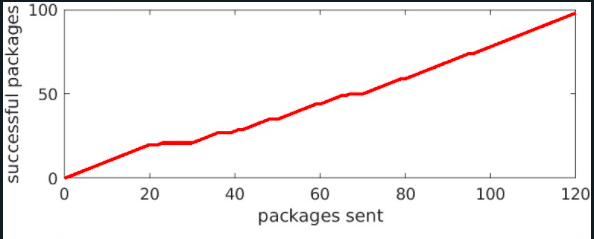
\includegraphics[width=0.3\textwidth]{gra.png}
    \centering
    \caption{Plot in matlab of practice 2}
    \label{fig:my_label6}
\end{figure}

\begin{figure}[h]
    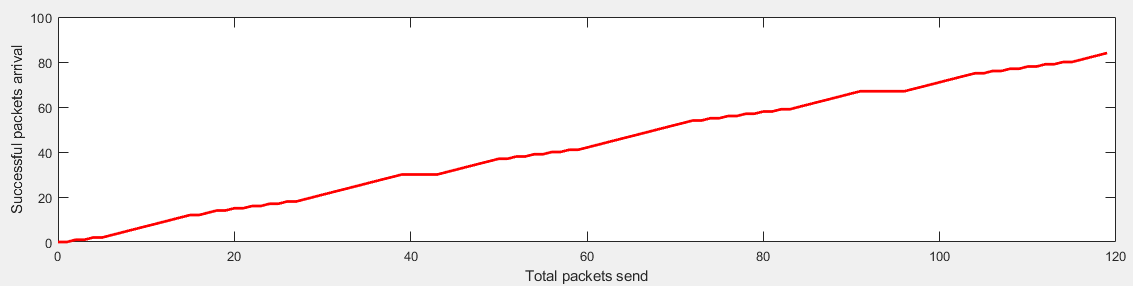
\includegraphics[width=0.3\textwidth]{plot1.PNG}
    \centering
    \caption{Plot in matlab of this practice}
    \label{fig:my_label6}
\end{figure}

\section{\textbf{CONCLUSIONS}}

\begin{itemize}

\item \textbf{Bonilla García Jesús Hernán}
In this project certain knowledge was applied, some of which had been working theoretically and others completely new, in my case it was a project that cost quite a lot of work since not leaving in a certain way had to try in another way, having than to research things about Arduino, also since it is a subject that costs a little more to obtain documentation or information on certain things, such as coding that was needed in the Arduino, since certain parts of programming and hardware had to be investigated as such
on this microcontroller, but with the help and union of the team it was possible to reach a result end by supporting us with experience or researching to reach our goal.

\item \textbf{González García Alan Alberto}
The complement provided by this practice implementing the GoBackN ARQ protocol I consider that it works in a great way to give a broader perspective of the scope that these modules can have when using both error detection protocols as well as error correction protocols, due to the complexity of the different error correction protocols we used the already mentioned with a fairly simple scale so as not to have many problems at the time of coding.


\item \textbf{Granados Bello Martin Alejandro}
This project helped us to ground the fundamentals acquired in the theoretical part of the course, because throughout this period we have studied some properties and definitions of the methods for error detection when establishing a communication between receiver and transmitter, and as a final result, we managed to capture in this practice one of the most essential. Such is the example of According to the work done, I could notice certain criteria that in my GoBackN. part were rusting, such as the connections that we use in the arduinos, which was a crucial part in the result of this practice because we had certain problems between the compatibility between these but which did not affect to obtain the final result.


\item \textbf{Gutiérrez Herrera Andrea}
At the end of the practice we understood the idea of Go-Back-N since they are protocols that adhere to the first ones we saw, they help us to better understand the idea of data transfer in the transport layer of computer networks. Using Arduinos we could physically see this since we had only seen it written and thus we can better understand the protocol


\item \textbf{Vega Barbosa Angel Josuhe}
In this practice, a joint work was carried out with the topics previously seen, such as CRC, but it was possible to see what applications could be taken to the data structures since to carry out the work of GoBack, which is a specific stay of the request protocol auto-repeat where the sending process continues to send frames specified by a window size even without receiving an ACK confirmation packet from the receiver. Everything could be done with satisfaction although there were complications due to the Arduino modules.
\end{itemize}
\section{\textbf{Bibliography}}

\begin{itemize}
\item \textbf{Fernández, L. (2020, 21 marzo). Protocolos de redes: la guía completa con todos los protocolos básicos. RedesZone.}
https://www.redeszone.net/tutoriales/internet/protocolos-basicos-redes/
\item \textbf{Polynomial codes for error detection. (2018). Computing.}
https://www.computing.dcu.ie/%7Ehumphrys/Notes/Networks/data.polynomial.html

\item \textbf{Wikipedia contributors. (2021, 11 marzo). Cyclic redundancy check. Wikipedia.}

https://en.wikipedia.org/wiki/Cyclicredundancycheck#
\item \textbf{Arduino Tutorials for Beginners. (s. f.). Arduino Getting Started.}
https://arduinogetstarted.com/

\item \textbf{Arduino Reference - Arduino Reference. (s. f.). Arduino.}
https://www.arduino.cc/reference/en/

\item \textbf{ASCII text,Hex,Binary,Decimal,Base64 converter. (s. f.). ASCII. }
https://www.rapidtables.com/convert/number/ascii-hex-bin-dec-converter.html
\item \textbf{Online CRC-8 CRC-16 CRC-32 Calculator. (s. f.). CRC.}
https://crccalc.com/

\end{itemize}
\section{\textbf{Appendix}}

\begin{itemize}

\item \textbf{TxGoBackN Arduino}
#include <RF24Network.h>          //Libraries
#include <RF24.h>
#include <SPI.h>
#include <stdio.h>
#include <stdlib.h>
#include <string.h>
RF24 radio (9,10);                 //Select pins for connection

RF24Network network(radio);

const uint16_t this_node = 01;      //Select number of nodes
const uint16_t other_node = 00;

typedef struct Nodo
{
    char dato[50];
    struct Nodo *siguiente;
} Nodo;

Nodo * crearNodo(char *d )
{
    Nodo *nuevo;
    nuevo = (Nodo*) malloc(sizeof(Nodo));
   strcpy(nuevo -> dato,d);
    nuevo -> siguiente=NULL;
    return nuevo;
}

Nodo * insertar(Nodo *cima,char *d)
{
    Nodo *nuevo;
    nuevo=crearNodo(d);
 Nodo * aux=cima;
    if(cima==NULL){
    return nuevo;

    }else{
      while(aux->siguiente!=NULL){

        aux=aux->siguiente;


      }
      aux->siguiente=nuevo;
      return cima;
    }
}

void verFila(Nodo *cima)
{
    Nodo *aux;
    aux = cima;

   if(aux==NULL)
    {
        Serial.println("La Fila esta vacia");
        return 1;
    }

    while(aux!=NULL)
    {

        Serial.println("Fila");
        Serial.println(aux->dato);
        aux=aux->siguiente;
    }
    return 0;
}



void setup() {                      //Connection settings
  Serial.begin(9600);
  SPI.begin();
  radio.begin();
radio.setDataRate(RF24_1MBPS);
radio.setPALevel(RF24_PA_MAX) ;
  network.begin(90,this_node);
  delay(5000);
  //Serial.println("Base station OK");
  
}


char *MakeCRC(char *BitString)
   {
   static char Res[6];                                 // CRC Result
   char CRC[5];
   int  i;
   char DoInvert;
   
   for (i=0; i<5; ++i)  CRC[i] = 0;                    // Init before calculation
   
   for (i=0; i<strlen(BitString); ++i)
      {
      DoInvert = ('1'==BitString[i]) ^ CRC[4];         // XOR required

      CRC[4] = CRC[3];
      CRC[3] = CRC[2];
      CRC[2] = CRC[1] ^ DoInvert;
      CRC[1] = CRC[0];
      CRC[0] = DoInvert;
      }
      
   for (i=0; i<5; ++i)  Res[4-i] = CRC[i] ? '1' : '0'; // Convert binary to ASCII
   Res[5] = 0;                                         // Set string terminator

   return(Res);
   }

    void Enviar(char *msj){
    char mensaje[15];
    strcpy(mensaje,msj);
 bool okComandoEnviado=false;
  network.update();
  RF24NetworkHeader headerMensaje(other_node);
   okComandoEnviado = network.write(headerMensaje,&mensaje,sizeof(mensaje));

  if(okComandoEnviado){

    //Serial.println("Comand sent");
   // Serial.print("El mensaje enviado es:");
    //Serial.println(mensaje);
    }else{
     // Serial.println("Comand NOT sent");
         //Serial.print("El mensaje NO enviado es:");
    //Serial.println(mensaje);
      }

  
  }

  int recibir(){

  
    char msjrecibido[15]="";
  bool ok2=false;
  int numerorecibido;  

    //Serial.print("Mensajes totales recibidos :");

 network.update();
 while(network.available()){
  if(network.available() > 0){
    RF24NetworkHeader headermsjrecibido;
    ok2=network.read(headermsjrecibido,
    &numerorecibido,sizeof(numerorecibido));

    }
  }
   
if(ok2){

  Serial.print("Mensaje recibido : ");
Serial.println(numerorecibido);
return numerorecibido;
    
  }else{

    Serial.println("Mensaje no recibido ");
    return 0;
    }


  
  }

  char *stbit(char *binario){
        char mensaje[15];
    strcpy(mensaje,binario);
    int dim=strlen(mensaje); 
     static char tam[50];
     char *Data;
     int n=0;
     for(byte j=0;j<dim;j++){                //Read the message bit by bit to write it to a string of characters
    for(int i=7;i>=0;i--){
      tam[n]=bitRead(mensaje[j],i)+'0';  
      n++;
     
        }
      }
      tam[n]='\0';
     Data=tam;  
    return tam;
    }

char *proces(char *mensaje){
    char binario[10];
     strcpy(mensaje,binario);
 
  
    char  *Result;
    char *Data;
     Data=stbit(binario);                                
   Result = MakeCRC(Data);                     //Calculate CRC-5-USB               

    //Serial.print("Mensaje:");
  //Serial.println(Data); 
  //Serial.print("CRC:");
 // Serial.println(Result);
  strcat(binario,Result);

//Serial.print("Mensaje a enviar:");
  //Serial.println(binario);
  return binario;
  }
   

void loop() {
  char binario[10]={"Hola"};
 
  
    char  *Result;
    char *Data;
     Data=stbit(binario);                                
   Result = MakeCRC(Data);                     //Calculate CRC-5-USB               

   // Serial.print("Mensaje:");
  //Serial.println(Data); 
  //Serial.print("CRC:");
  //Serial.println(Result);
  strcat(binario,Result);

//Serial.print("Mensaje a enviar Final:");
  //Serial.println(binario);
  

Nodo *Cima;
Cima=NULL;

Cima=insertar(Cima,binario);
Cima=insertar(Cima,binario);
Cima=insertar(Cima,binario);
Cima=insertar(Cima,binario);
Cima=insertar(Cima,binario);
Cima=insertar(Cima,binario);

//Serial.print("Fila:");
//verFila(Cima);

int j=1;
int ack=0;
int ack2=0;
 Nodo *aux;
    aux = Cima;
 
    while(aux!=NULL)
    {
   
      if(aux->siguiente==NULL){
       // Serial.println("Ultimo paquete");
        Enviar(aux->dato);
        delay(500);
       ack=recibir();
        delay(500); 
            if(ack==1){
 
              aux=aux->siguiente;
              //Serial.print("mov ventana:");
              //Serial.println(j);
              j++;
       
              }
        }else{
             Enviar(aux->dato);
        delay(500); 
      Enviar(aux->siguiente->dato);
        
        delay(500); 
         ack=recibir();
    delay(500); 
    ack2=recibir();
    delay(500); 
    if(ack==1){
 
              aux=aux->siguiente;
              //Serial.print("mov ventana:");
              //Serial.println(j);
              j++;
      
              if(ack2==1){
        
                aux=aux->siguiente;
              // Serial.print("mov ventana:");
              //Serial.println(j);
              j++;
  
                        }   
              }
        }    
    }
  
}
\item \textbf{RxGoBackN Arduino}
#include <RF24Network.h>        //Libraries
#include <RF24.h>
#include <SPI.h>
#include <stdio.h>
#include <stdlib.h>
#include <string.h>
RF24 radio (9,10);              //Select pins for connection

RF24Network network(radio);

const uint16_t this_node = 00;         //Select number of nodes
const uint16_t other_node = 01;

void setup() {                        //Connection settings
  Serial.begin(9600);
   SPI.begin();
  radio.begin();
radio.setDataRate(RF24_1MBPS);
radio.setPALevel(RF24_PA_MAX) ;
  network.begin(90,this_node);
  delay(5000);
  //Serial.println("Base station OK");

}

int msjSend=0;
int msjSucces=0;


char *MakeCRC(char *BitString)
   {
   static char Res[6];                                 // CRC Result
   char CRC[5];
   int  i;
   char DoInvert;
   
   for (i=0; i<5; ++i)  CRC[i] = 0;                    // Init before calculation
   
   for (i=0; i<strlen(BitString); ++i)
      {
      DoInvert = ('1'==BitString[i]) ^ CRC[4];         // XOR required?

      CRC[4] = CRC[3];
      CRC[3] = CRC[2];
      CRC[2] = CRC[1] ^ DoInvert;
      CRC[1] = CRC[0];
      CRC[0] = DoInvert;
      }
      
   for (i=0; i<5; ++i)  Res[4-i] = CRC[i] ? '1' : '0'; // Convert binary to ASCII
   Res[5] = 0;                                         // Set string terminator

   return(Res);
   }


int recibir(){
 char msjrecibido[10]="";
  int ack=1;
    bool ok2=false;
   network.update();                 //Reception of sent message
    while(network.available()){
      if(network.available() > 0){
    RF24NetworkHeader headermsjrecibido;
    ok2=network.read(headermsjrecibido,&msjrecibido,sizeof(msjrecibido));

    }
  }
   
if(ok2){                              //Message receipt validation
  //Serial.print("Mensaje recibido con CRC es: ");
  //Serial.println(msjrecibido);
  int dim=strlen(msjrecibido)-5;
  int mov=dim;
  char *Crc = "";
  
char  Result[2];
    char tam[50];
    char tam2[6];
    char *Data;
    int n=0;
    char txcrc[6]="";
    for(int i=0;i<5;i++){       //Store the CRC of the received message in a character string
txcrc[i]=msjrecibido[mov];
mov++;    

      }
msjrecibido[dim]=0;         //Remove the CRC of the message

  // Serial.print("Mensaje recibido sin CRC es: ");
  //Serial.println(msjrecibido);
  //Serial.print(" CRC en mensaje es: ");
 //Serial.println(txcrc);

    for(byte j=0;j<dim;j++){             //Read the message bit by bit to write it to a string of characters
    for(int i=7;i>=0;i--){
      tam[n]=bitRead(msjrecibido[j],i)+'0';  
      n++;
     
        }
      }
      tam[n]='\0';
     Data=tam;  

  

 Crc = MakeCRC(strcat(Data,txcrc));               //Calculate CRC-5-USB 
    //Serial.print("Mensaje Recibido en binario:");
  //Serial.println(Data); 

//  Serial.print("TxCRC:");
//  Serial.println(txcrc);
   //Serial.print("RxCRC:");
     //Serial.println(Crc);

if( strcmp("00000", Crc) == 0) //Comparison and validation of received CRC with the calculated one
{
  // Serial.println("Mensaje Recibido Correctamente dado crc es 0 enviando ACK");
  msjSucces++;
   return 1;
    
  }else{
    
    //Serial.println("Mensaje Recibido Con error dado  crc no es 0 enviando NACK");
   return 0; 
    }
  
  }else{
    //Serial.println("Mensaje no recibido ");
     return 0; 
    }
  
  }


 void Enviar(int msj){

      int ack=msj;
    bool okComandoEnviado=true;

  network.update();
  RF24NetworkHeader headerMensaje(other_node);
  okComandoEnviado = network.write(headerMensaje,&ack,sizeof(ack));

  if(okComandoEnviado){

    //Serial.println("Comand sent");
    //Serial.print("El mensaje enviado es:");
    //Serial.println(msj);
    }else{
      //Serial.println("Comand NOT sent");
         //Serial.print("El mensaje NO enviado es:");
    //Serial.println(msj);
      }

  
  }




void loop() {
 
   
  int ack=recibir();
  msjSend++;
  Serial.print(msjSucces);
//Serial.print("\t");
  //Serial.print(msjSend); 
  //Serial.print("Ack o NAck");
    //Serial.println(ack);
          delay(500);
              Serial.print("\n");
  int ack2=recibir();
  msjSend++;
  Serial.print(msjSucces);
//Serial.print("\t");
 // Serial.print(msjSend); 
  //Serial.print("Ack o NAck");
    //Serial.println(ack2);
          delay(500);
          
          Enviar(ack);
  //Serial.print(msjSend); 
    //Serial.print("\n");
          delay(500);
          Enviar(ack2);
//Serial.print(msjSend); //Mensajes Totales totales enviados
    Serial.print("\n");
          delay(500);

  
    
}


\end{itemize}


\end{document}

